% vim: set spell spelllang=en tw=100 et sw=4 sts=4 :

\documentclass{llncs}

% \usepackage{showframe}

\usepackage{times}
\usepackage{complexity}
\usepackage{hyperref}
\usepackage{microtype}
\usepackage{xcolor,colortbl}
\usepackage{tabularx}
\usepackage{siunitx}
\usepackage{xspace}
\usepackage{scalefnt}
\usepackage{graphicx}
\usepackage{booktabs}

\newcommand{\VFtwo}{$\textsc{Vf{\scalefont{0.8}2}}$\xspace}
\newcommand{\Glasgow}{$\textsc{Glasgow}$\xspace}
\newcommand{\LAD}{$\textsc{Lad}$\xspace}
\newcommand{\IncompleteLAD}{$\textsc{IncompleteLad}$\xspace}
\newcommand{\PathLAD}{$\textsc{PathLad}$\xspace}
\newcommand{\GlasgowOne}{$\textsc{Glasgow{\scalefont{0.8}1}}$\xspace}
\newcommand{\GlasgowTwo}{$\textsc{Glasgow{\scalefont{0.8}2}}$\xspace}
\newcommand{\GlasgowThree}{$\textsc{Glasgow{\scalefont{0.8}3}}$\xspace}
\newcommand{\GlasgowFour}{$\textsc{Glasgow{\scalefont{0.8}4}}$\xspace}
\newcommand{\LLAMA}{$\textsc{Llama}$\xspace}

\title{Portfolios of Subgraph Isomorphism Algorithms}

\author{
    Lars Kotthoff\inst{1}
    \and Ciaran McCreesh\thanks{This work was supported by the Engineering
        and Physical Sciences Research Council [grant number EP/K503058/1]}\inst{2}
    \and Christine Solnon\inst{3}}

\institute{
    University of British Columbia, Vancouver, Canada
    \and University of Glasgow, Glasgow, Scotland
    \and INSA-Lyon, LIRIS, UMR5205, F-69621, France}

\begin{document}

\maketitle

\begin{abstract}
Subgraph isomorphism is a computationally challenging problem with important practical
applications, for example in computer vision, biochemistry, and model checking. There are a number
of state-of-the-art algorithms for solving the problem, each of which has its own performance
characteristics. As with many other hard problems, the single best choice of algorithm overall is
rarely the best algorithm on an instance-by-instance. We develop a portfolio approach which leverages
novel features to characterise subgraph isomorphism problems to dynamically decide which algorithm
to use on a per-instance basis. We demonstrate significant performance improvements on a large set
of hard benchmark problems. In addition, we show how algorithm selection models can be leveraged to
gain new insights into what affects the performance of an algorithm.
\end{abstract}

\section{Introduction}

The subgraph isomorphism problem is to find an adjacency-preserving injective mapping from vertices
of a small \emph{pattern} graph to vertices of a large \emph{target} graph. This \NP-complete
problem has many important practical applications, for example in computer vision
\cite{cviu11,pr15}, biochemistry \cite{Giugno:2013}, and model checking \cite{Sevegnani:2015}. There
exist various exact algorithms, which have been compared on a large suite of problem instances by
McCreesh and Prosser \cite{McCreesh:2015}. These experiments indicated that the single best
algorithm depends on the CPU time limit considered: for very small CPU time limits, \VFtwo
\cite{Cordella:2004} is the best choice, whereas the \Glasgow algorithm \cite{McCreesh:2015} has
better success rates for larger time limits.  They also showed that on an instance by instance
basis, other algorithms are often better.

In this paper, we report experimental results on a larger set of 8 algorithms, including new
variants, and a larger benchmark. We show that 4 of these algorithms are single best algorithms,
depending on the CPU time limit considered, and that combining preprocessing with an algorithm
selection on an instance by instance basis allows us to achieve better overall performance than any
single algorithm.

\section{Definitions and Notations}

A \emph{graph} $G=(N,E)$ consists of a \emph{node set} $N$ and an \emph{edge set} $E \subseteq N
\times N$, where an edge $(u,u')$ is a pair of nodes. The number of neighbors of a node $u$ is
called the degree of $u$, $d^\circ(u)=\#\{ (u,u')\in E\}$. In this paper, we implicitly consider
non-directed graphs, such that $(u,u')\in E\Leftrightarrow (u',u)\in E$. The extension to directed
graphs is rather straightforward, and all algorithms compared in this paper can handle directed
graphs as well.

Given a pattern graph $G_p=(N_p,E_p)$ and a target graph $G_t=(N_t,E_t)$, the \emph{subgraph
isomorphism problem} consists of deciding whether $G_p$ is isomorphic to some subgraph of $G_t$.
More precisely, the goal is to find an injective matching $f: N_p\rightarrow N_t$, that associates a
different target node to each pattern node, and that preserves pattern edges, i.e.\ $\forall (u,u')
\in E_p, (f(u),f(u')) \in E_t$.

Note that the subgraph is not necessarily induced, so that two pattern nodes that are not linked by
an edge may be mapped to two target nodes which are linked by an edge. This problem is also called
\emph{subgraph monomorphism} or \emph{subgraph matching} in the literature.

In the following, we assume $G_p=(N_p,E_p)$ and $G_t=(N_t,E_t)$ to be the underlying instance of a
subgraph isomorphism problem.  We also define $n_p = \# N_p$, $n_t = \# N_t$,  $e_p=\# E_p$, $e_t=\#
E_t$, and $d_p$ and $d_t$ to be the maximum degrees of the graphs $G_p$ and $G_t$.

\section{Subgraph Isomorphism Algorithms}

Subgraph isomorphism problems may be solved by a systematic exploration of the search space composed
of all possible injective matchings from $N_p$ to $N_t$: starting from an empty matching, one
incrementally extends a partial matching by matching a non-matched pattern node to a non-matched
target node until either some edges are not matched by the current matching (so the search must
backtrack to a previous choice point and go on with another extension), or all pattern nodes have
been matched (a solution has been found). To reduce the search space, this exhaustive exploration is
combined with filtering techniques that aim at removing candidate pairs of non-matched
pattern-target nodes $(u,v)\in N_p\times N_t$. Different filtering techniques may be considered;
some are stronger than others (they remove more candidate pairs), but also have higher time
complexities.

\subsection{Filtering for Subgraph Isomorphism}

The simplest form of filtering is simply to propagate difference constraints (which ensure that the
matching is injective) and edge constraints (which ensure that the matching preserves pattern
edges): each time a pattern node $u\in N_p$ is matched with a target node $v\in N_t$, one removes
every candidate pair $(u',v')\in N_p\times N_t$ such that either $v'=v$ (difference constraint) or
$(u,u')$ is a pattern edge but $(v,v')$ is not a target edge (edge constraint). This simple
filtering (called \emph{Forward-Checking}) is very fast to achieve: in ${\cal O}(n_p)$ for
difference constraints, and in ${\cal O}(d_p\cdot n_t)$ for edge constraints. It is used, for
example, in McGregor's algorithm \cite{mcgregor79} and in \VFtwo \cite{Cordella:2004}.

R\'egin \cite{regin} introduced a stronger filtering for difference constraints, which ensures that
all pattern nodes can be matched with different target nodes, all together. This filtering (called
\emph{All-Different Generalized Arc Consistency}) removes more candidate pairs than when each
difference constraint is propagated separately which Forward-Checking. However, it is also more time
consuming as it is done in ${\cal O}(n_p^2\cdot n_t^2)$ time.

Various filtering techniques have been tried for edge constraints. Ullman \cite{ullman} introduced a
filtering which ensures that for each pattern edge $(u,u')\in E_p$ and each candidate pair $(u,v)\in
N_p\times N_t$, there exists a candidate couple $(u',v')\in N_p\times N_t$ such that $(v,v')$ is a
target edge. Candidate couples $(u,v)$ that do not satisfy this property are iteratively removed
until a fixed point is reached. This filtering (called \emph{Arc Consistency}) removes more
candidate pairs than Forward-Checking, but it is also more time consuming as it is done in ${\cal
O}(e_p\cdot n_t^2)$ when using the algorithm AC4  \cite{MH86}.

Stronger filtering may be obtained by propagating edge constraints in a more global way, as proposed
by Larrosa and Valiente \cite{LV02}. The idea is to check for each candidate pair $(u,v)\in
N_p\times N_t$ that the number of pattern nodes adjacent to $u$ is smaller than or equal to the
number of target nodes that are both adjacent to $v$ and that may be matched with nodes adjacent to
$u$. This is done in ${\cal O}(n_p^2\cdot n_t^2)$. This idea was generalised by Solnon
\cite{Solnon:2010}'s \LAD algorithm, where, for each candidate pair $(u,v)\in N_p\times N_t$, a redundant Local
All-Different constraint ensures that each neighbour of $u$ may be matched with a different
neighbour of $v$. This is done in ${\cal O}(n_p\cdot n_t\cdot d_p^2\cdot d_t^2)$.

\subsection{Propagation of Invariant Properties}

Some filtering techniques exploit invariant properties, i.e.\ properties associated with nodes such
that nodes may be matched only if they have compatible properties. A classical property is the
degree: a pattern node $u\in N_p$ may be matched with a target node $v\in N_t$ only if
$d^\circ(u)\leq d^\circ(v)$. This property is usually used at the beginning of the search to reduce
the set of candidate pairs to $\{(u,v)\in N_p\times N_t\;|\;d^\circ(u)\leq d^\circ(v)\}$.  Other
examples of invariant properties are the number of cycles of length $k$ passing through the node,
and the number of cliques of size $k$ containing the node, which must be smaller for a pattern node
than for its matched target node.  Invariant properties may also be associated with pairs of nodes.
For example, the number of paths of length $k$ between two pattern nodes is smaller than or equal to
the number of paths of length $k$ between the target nodes with which they may be matched.

These invariant properties are used, for example:

\begin{itemize}
\item  By Battiti and Mascia \cite{battiti-mascia07}, to remove candidate pairs $(u,v)\in N_p\times
    N_t$ such that the number of paths starting from  pattern node $u$ is greater than the number of
    paths starting from  target node $v$;
\item By Audemard et al.\ \cite{Audemard:2014} to generalise the locally all-different constraint
    proposed by Solnon \cite{Solnon:2010} so that it ensures that a subset of pattern nodes can be
    matched with all different compatible target nodes, where compatibility is defined with respect
    to invariant properties;
\item by McCreesh and Prosser \cite{McCreesh:2015} to filter the set of candidate couples before
    starting the search, and to generate additional implied adjacency-like constraints which are
    processed during search.
\end{itemize}

\noindent Audemard et al.\ \cite{Audemard:2014} do not limit the length of paths considered, and
iteratively increment the length until no more pairs are removed. Battiti and Mascia
\cite{battiti-mascia07}, and McCreesh and Prosser \cite{McCreesh:2015} parameterise their algorithms
by the maximum path length considered when counting paths: larger values for this parameter remove
more candidate pairs, but are also more time consuming. Battiti and Mascia's experiments show that
the best setting depends on the instance considered, and that a portfolio running several randomised
versions in time-sharing decreases the total CPU time needed to find a solution for feasible
instances. McCreesh and Prosser simply set the parameter to 3, as this setting seemed to be a
reasonable compromise.

\subsection{Per-Instance Algorithm Selection}

The per-instance algorithm selection problem~\cite{rice_algorithm_1976} is to select from an
algorithm portfolio~\cite{huberman_economics_1997,gomes_algorithm_2001} the one expected to perform
best on a given problem instance. Algorithm selection systems usually build machine learning models
of the algorithms or the in which portfolio they are contained to forecast which algorithm to use in a
particular context. Using the model predictions, one or more algorithms from the portfolio are
selected to be run sequentially or in parallel.

Here, we consider the case where exactly one algorithm is selected for solving the problem. One of
the most prominent and successful systems that employs this approach is
SATzilla~\cite{xu_satzilla_2008}, which defined the state of the art in SAT solving for a number of
years. Other application areas include constraint solving~\cite{omahony_using_2008}, the travelling
salesperson problem~\cite{kotthoff_improving_2015}, and AI planning~\cite{seipp_learning_2012}.
The interested reader is referred to a recent survey~\cite{kotthoff_algorithm_2014} for additional
information on algorithm selection.

\subsection{Problem Instances}

We consider 5725 instances, which are available in a simple text
format\footnote{\url{http://liris.cnrs.fr/csolnon/SIP.html}}. These instances are grouped into 12
classes.

\begin{itemize}
\item Class 1 contains randomly generated scale-free graphs \cite{constraints10}.
\item Classes 2 and 3 contain various kinds of graphs selected by Larrosa and Valiente \cite{LV02}:
    class 2 contains small instances generated from the 50 first graphs, and class 3 contains
    larger instances where pattern graphs are coming from class 2, and target graphs are coming from
    the next 50 graphs.
\item Classes 4 to 8 contain randomly generated graphs coming from a database of graphs commonly
    used for benchmarking subgraph isomorphism algorithms
    \cite{GraphDatabase1,GraphDatabase2}: bounded-degree graphs for classes 3 and 4, regular meshes
    for classes 5 and 6, and random graphs with uniform edge probabilities for class 7. All of these
    instances are satisfiable.
\item Classes 9 and 10 contain instances coming from segmented images \cite{pr15,cviu11}.
\item Class 11 contains instances coming from meshes modeling 3D objects \cite{cviu11}.
\item Class 12 contains random graph instances chosen to be close to the satisfiable-unsatisfiable
    phase transition---these instances are expected to be particularly challenging, despite their
    small size.
\end{itemize}

Note that Classes 3 and 12 were not considered in the previous experimental study by McCreesh and
Prosser \cite{McCreesh:2015}.  This set of instances is also much larger than that of Battiti and
Mascia~\cite{battiti-mascia07}, who were the first to propose algorithm portfolios for subgraph
isomorphism problems.  Battiti and Mascia only considered a pure parallel portfolio consisting of
two solvers, and without a selection mechanism. Their problem set consisted entirely of easy
satisfiable instances, which is where this style of approach has most success.

\subsection{Experimental Setup}

We measured runtimes on machines with Intel Xeon E5-2640 v2 CPUs and 64GBytes RAM, running
Scientific Linux 6.5. We used the C++ implementation of the \Glasgow algorithm \cite{McCreesh:2015},
the C implementation of \LAD \cite{Solnon:2010}, and the VFLib C implementation of \VFtwo
\cite{Cordella:2004}. Software was compiled using GCC 4.9. Each problem instance was run with a
timeout of $10^8$ milliseconds (a little over a day).

\subsection{Portfolio Composition}

We have selected a set of algorithms with complementary performance:
\begin{itemize}
\item \VFtwo \cite{Cordella:2004}, which performs a weak filtering that it is especially fast on
    trivially satisfiable instances;
\item \LAD \cite{Solnon:2010}, which combines two strong but expensive filtering techniques
    (All-Different Generalized Arc Consistency and Locally All-Different);
\item \Glasgow \cite{McCreesh:2015}, which does expensive preprocessing based on path length
    invariant properties to generate additional constraints, followed by weaker filtering
    (forward-checking, and a heuristic All-Different propagator which can miss deletions) and
    conflict-directed backjumping during search.
\end{itemize}

\noindent The \Glasgow algorithm has a parameter, which controls the lengths of paths used when
reasoning about non-adjacent vertices.  In experiments reported by McCreesh and Prosser
\cite{McCreesh:2015}, the choice of paths of length 3 was used as a reasonable compromise---longer
paths lead to prohibitively expensive preprocessing on larger, denser instances. This is often not
the best choice on an instance by instance basis: sometimes path-based reasoning gives no benefit at
all, sometimes considering only paths of length 2 suffices, occasionally paths of length 4 are
helpful, and even looking at paths of length 3 is relatively expensive on some graphs. We thus all
four choices, naming these variants \GlasgowOne through \GlasgowFour.

We also introduce two new variants of \LAD. The first, called \IncompleteLAD, is a weaker
filtering which is applied once, without performing a backtracking search, and very quickly
detects inconsistencies on many instances: for each pattern node $u$, we check that there exists at
least one target node $v$ such that for each neighbor $u'$ of $u$ there exists a different neighbor
$v'$ of $v$ such that the degree of $u'$ is smaller than or equal to the degree of $v'$.
\IncompleteLAD is an incomplete algorithm as it can only detect inconsistency of some instances: when
it does not detect inconsistency, the instance may either be satisfiable or not. As a counterpart of
this incompleteness, it is very fast: its time complexity is ${\cal O}(n_p(n_t+e_t))$.

The second variant of \LAD is called \PathLAD, which combines the locally all-different constraints
introduced by Solnon \cite{Solnon:2010} with the exploitation of path length properties proposed by
Audemard et al.\ \cite{Audemard:2014}. The idea is to label each edge $(u,v)$ with the number of
paths of length 2 between $u$ and $v$, and each node $u$ with the number of cycles of length 3
passing through $u$, and to add the constraint that the label of a pattern node (resp.\ edge) must
be smaller than or equal to the label of its associated target node (resp.\ edge).

\subsection{Results for Individual Algorithms} \label{expComp}

\begin{figure}[t]
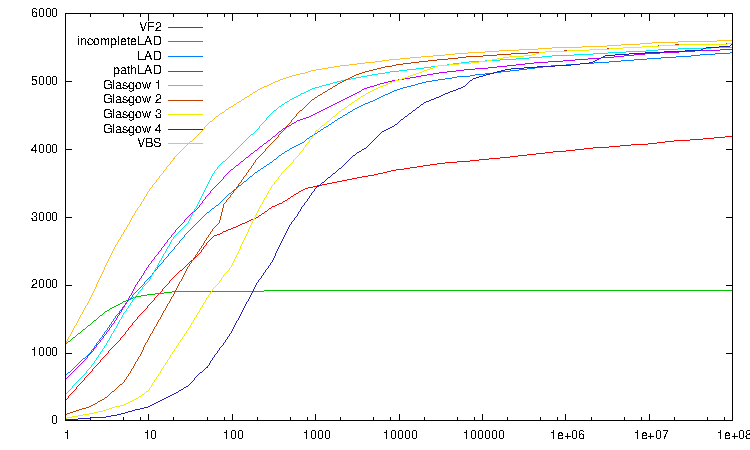
\includegraphics[width=\textwidth]{courbe.pdf}
\caption{Evolution of the number of solved instances with respect to CPU time, for the 8 algorithms
of the portfolio, and a Virtual Best Solver (VBS).\label{expTimeGraph}}
\end{figure}

Figure \ref{expTimeGraph} displays the evolution of the number of instances solved with respect to
CPU time. It shows us that the best solver depends on the time limit considered. \IncompleteLAD is
able to solve easy unsatisfiable instances very quickly, in a few milliseconds. Hence, for time
limits lower than \SI{5}{\ms}, the best solver is \IncompleteLAD. However, it is not able to solve harder
unsatisfiable instances, nor can it solve satisfiable instances.

\PathLAD and \GlasgowOne outperform \IncompleteLAD when considering longer time limits: \PathLAD is the
best solver for time limits larger than \SI{5}{\ms} and lower than \SI{40}{\ms}, and \GlasgowOne is the best solver
for time limits larger than \SI{40}{\ms} and lower than \SI{3000}{\ms}.

For CPU time limits larger than \SI{3000}{\ms}, the best solver becomes \GlasgowTwo.  As we
increase the CPU time limit, variants of \Glasgow with longer paths (\GlasgowThree and \GlasgowFour)
become better. This is what we expect, as more reasoning is expensive, but potentially increases the
reduction of the search space. In particular, the relative performance of Glasgow variants is
monotone in the time it takes to solve the instance---\GlasgowOne is best at first, but gets worse as
the time to solve the instance increases until \GlasgowTwo is better. After that point, \GlasgowOne is
never better than \GlasgowTwo again. The same is true for path lengths 3 and 4.

The figure illustrates the potential for portfolios and algorithm selection we have. There is
clearly no single solver that dominates throughout.

Furthermore, the Virtual Best Solver (VBS), which considers the best algorithm for each instance
separately, obtains much better results, showing us that the algorithms have complementary
performance. The difference between VBS and single best is more particularly important for rather
small CPU time limits (smaller than \SI{1000}{\ms}). In many applications, it is important to have the
fastest possible algorithm. For example, in pattern recognition \cite{pr15,cviu11} and chemical
\cite{Giugno:2013} applications, we often have to solve the subgraph isomorphism problem repeatedly
for a very large number of graphs (in order to find a pattern image or molecule in a large database
of target images or compounds, for example), so having an algorithm that is able to solve an
instance in \SI{100}{\ms} instead of \SI{1000}{\ms} makes a big difference.  Therefore, it is important to select
the best algorithm for each instance, even if the instance is an easy one.

Table~\ref{expClass} shows us that we cannot simply select algorithms based upon which class from
which instances are coming (unlike in SAT, where this kind of approach can be reasonable). For all
classes, there are always at least two algorithms which are the best for at least one instance of
the class. In particular, for classes 2 and 3, each algorithm is the best for at least one instance
(except \GlasgowFour for class 3).

\begin{table}[t]
\begin{center}
\begin{tabularx}{.8\textwidth}{XXrXrrrXrrrr}
\toprule
Class && \VFtwo && \multicolumn{3}{c}{\LAD} && \multicolumn{4}{c}{\hspace*{2em}\Glasgow}\\
&&&&incomplete&default&path&&1&2&3&4\\
\midrule
1 &&        0 &&       20 &        0 &        0 &&       80 &        0 &        0 &        0 \\
2 &&      201 &&       92 &      189 &      270 &&      520 &      180 &       53 &       15 \\
3 &&      112 &&     1608 &      617 &      959 &&      396 &      195 &       21 &        0 \\
4 &&      270 &&        0 &        0 &        0 &&        5 &        0 &        0 &        0 \\
5 &&      266 &&        0 &        1 &        3 &&       31 &        0 &        0 &        0 \\
6 &&       71 &&        0 &        0 &        0 &&        7 &       14 &        1 &        0 \\
7 &&      270 &&        0 &        0 &        0 &&        5 &        0 &        0 &        0 \\
8 &&        0 &&        0 &        0 &        1 &&      195 &       69 &        6 &        0 \\
9 &&       77 &&        3 &        0 &       19 &&      103 &        1 &        0 &        0 \\
10 &&       13 &&        0 &        2 &        2 &&        7 &        0 &        0 &        0 \\
11 &&        2 &&      142 &       71 &       17 &&       23 &        0 &        0 &        0 \\
12 &&        0 &&        0 &        1 &        2 &&      158 &        6 &        1 &        0 \\
\midrule
Total && 1282 && 1865 & 881 & 1273 && 1530 & 465 & 82& 15\\
\bottomrule
\end{tabularx}
\end{center}
\caption{Number of times each algorithm is best, for each class.\label{expClass}}
\end{table}

\section{Algorithm Selection Approach}

Our approach is composed of three steps. First, we run two presolvers in a static way to quickly
solve easy instances; second, we extract features from instances which are not solved by the first
step; and third, we select an algorithm and run it.

\subsection{Presolving}

Experimental results reported in Section~\ref{expComp} have shown us that \IncompleteLAD is very fast
(\SI{7}{\ms} on average) and is able to solve 1919 instances very quickly. Therefore, we first run
\IncompleteLAD: if the instance is detected to be unsatisfiable, then we do not process it further.
Otherwise, we record as features the number of candidate couples removed by \IncompleteLAD in absolute
terms, as a percentage, and the minimum and maximum on a per-variable basis.

\VFtwo is also able to solve many easy instances very quickly: among the 3806 instances which are not
solved by \IncompleteLAD, 1470 are solved by \VFtwo in less than 50 milliseconds. Therefore, after
running \IncompleteLAD, we run the \VFtwo solver for \SI{50}{\ms}. This solves easy instances without
the overhead of running algorithm selection and avoids potentially making incorrect solver choices.
After running \IncompleteLAD and \VFtwo for \SI{50}{\ms}, we are left with 2336 hard instances that we
consider for algorithm selection.

\subsection{Feature Extraction}

If presolving does not give us a solution, we extract additional features. For both the pattern and
the target graph, we consider some basic graph properties, which may be computed very quickly:

\begin{itemize}
    \item The number of vertices and edges.
    \item The density---we expect that some kinds of filtering might be expensive and ineffective on
        dense graphs.
    \item How many loops (self-adjacent vertices) the graph contains---since loops must be mapped to
        loops, this could have a strong effect on how easy an instance is.
    \item The mean and maximum degrees, and whether or not every vertex has the same degree. (The
        degree-based invariants used by \LAD and \Glasgow do nothing at the top of search if every
        vertex has the same degree.)
    \item Whether or not the graph is connected.
    \item The mean and maximum distances between all pairs of vertices (if nearly all vertices are
        close together, path-based reasoning is likely to be ineffective). We also consider the
        proportion of vertex pairs which are distance at least 2, 3 and 4 apart.
\end{itemize}

\subsection{Selection Model}

To decide which solver to run on the remaining instances, we use \LLAMA~\cite{kotthoff_llama_2013}.
\LLAMA supports the most common algorithm selection approaches used in the literature. We performed a
set of preliminary experiments to determine the approach that works best in this case.

We use 10-fold cross-validation to determine the performance of the \LLAMA models. The entire set of
instances was randomly partitioned into 10 subsets of approximately equal size. Of the 10 subsets, 9
were combined to form the training set for the algorithm selection models, which were evaluated on
the remaining subset. This process was repeated 10 times for all possible combinations of training
and test sets. At the end of this process, each problem instance in the original set was used
exactly once to evaluate the performance of the algorithm selection models.

\LLAMA's pairwise regression approach with random forest regression gave the best performance. The
idea is very similar to the pairwise classification used by Xu et al.\ \cite{xu_satzilla_2008}. For
each pair of algorithms in our portfolio, we train a model that predicts the performance difference
between them. That is, if the first algorithm is better than the second, the difference is positive,
otherwise negative. The algorithm with the highest cumulative performance difference, i.e.\ the most
positive difference over all other algorithms, is chosen to be run.

As this approach gives very good performance already, we did not tune the parameters of the random
forest machine learning algorithm. It is possible that overall performance can be improved by doing
so and we make no claims that the particular algorithm selection approach we use in this paper
cannot be improved.

The data we use in this paper is available as ASlib~\cite{aslib} scenario GRAPHS-2015.

\section{Experimental Evaluation of Algorithm Selection}

Table~\ref{tab:res} shows the performance of our algorithm selection approach, compared to two
baselines. The virtual best solver is the oracle predictor that, for each instance, chooses the best
solver from our portfolio. This is the upper bound of what an algorithm selection approach can
achieve. The single best solver is the one solver from the portfolio that has the overall best
performance across the entire set of instances, at the CPU time limit of \SI{e8}{\ms},
i.e.\ \GlasgowTwo. We consider it a lower bound on performance.
We are able to solve 34 more instances than the single best solver within the timeout, with only an
additional 13 to the virtual best. In terms of average performance, we are able to close almost
\SI{70}{\percent} of the gap between the single best and the virtual best solver.

\begin{table}[ht]
    \centering\setlength{\tabcolsep}{1em}
\begin{tabular}{lrrr}
  \toprule
model & mean MCP & solved instances & mean performance\\
  \midrule
virtual best & 0 & 2219 & 5822809\\
single best & 1965158 & 2172 & 7787967\\
\LLAMA & 610835 & 2206 & 6435301\\
   \bottomrule \\
\end{tabular}
\caption{Algorithm selection performance on the reduced set of 2336
instances. MCP is the misclassification penalty; that is, the additional time
required to solve a set of instances because of choosing solvers that perform
worse than the best.}\label{tab:res} \end{table}

Table~\ref{tab:res} shows the performance of the selection model. The performance of the entire
system we propose here is shown in Table~\ref{tab:resfull}. The additional instances are solved
either by \IncompleteLAD or \VFtwo presolving, as explained above. Our system is able to close more than
\SI{50}{\percent} of the gap between single and virtual best.

\begin{table}[ht]
    \centering\setlength{\tabcolsep}{1em}
\begin{tabular}{lrrr}
  \toprule
model & mean MCP & solved instances & mean performance\\
  \midrule
virtual best & 0 & 5608 & 2375913\\
single best & 798660 & 5562 & 3174573\\
\LLAMA & 249242 & 5595 & 2625831\\
   \bottomrule \\
\end{tabular}
\caption{Algorithm selection system performance on the full set of 5725
instances.}\label{tab:resfull}
\end{table}

Figure~\ref{fig:portfolio-ecdf} shows the cumulative distribution function for
the individual solvers, the virtual best solver, and the \LLAMA portfolio. The
virtual best solver clearly dominates with a significant margin to the next
best. \VFtwo is far below all other solvers. The portfolio does not perform well
for instances that can be solved quickly because of the overhead incurred
through feature computation. As the instances become more difficult to solve,
its performance improves.

\begin{figure}[!ht]
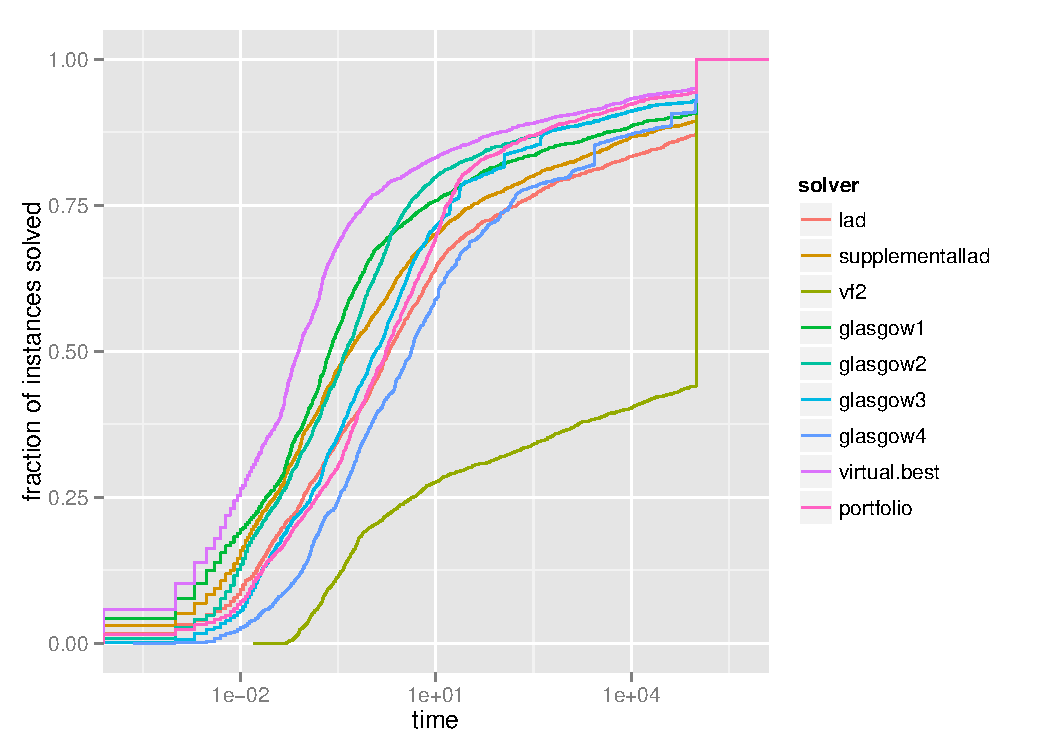
\includegraphics[width=\textwidth]{figures/portfolio-ecdf}
\caption{Empirical cumulative distribution function of solvers, virtual best
solvers, and the \LLAMA portfolio on the reduced set of 2336 instances. The
actual solvers are shown as dashed lines.}
\label{fig:portfolio-ecdf}
\end{figure}

Figure~\ref{fig:portfolio-ecdf-full} shows the ECDF of the system including
\IncompleteLAD and \VFtwo presolving on the full set of instances. Note that for
very easy instances, we are better than the virtual best solver because
\IncompleteLAD is not included in our portfolio. The performance on small
instances is much better than the \LLAMA selector alone (cf.\
Figure~\ref{fig:portfolio-ecdf}) and the region where the portfolio performs
worse than the individual solvers is now limited to approximately $10^2$ to
$10^4$ milliseconds.

\begin{figure}[!ht]
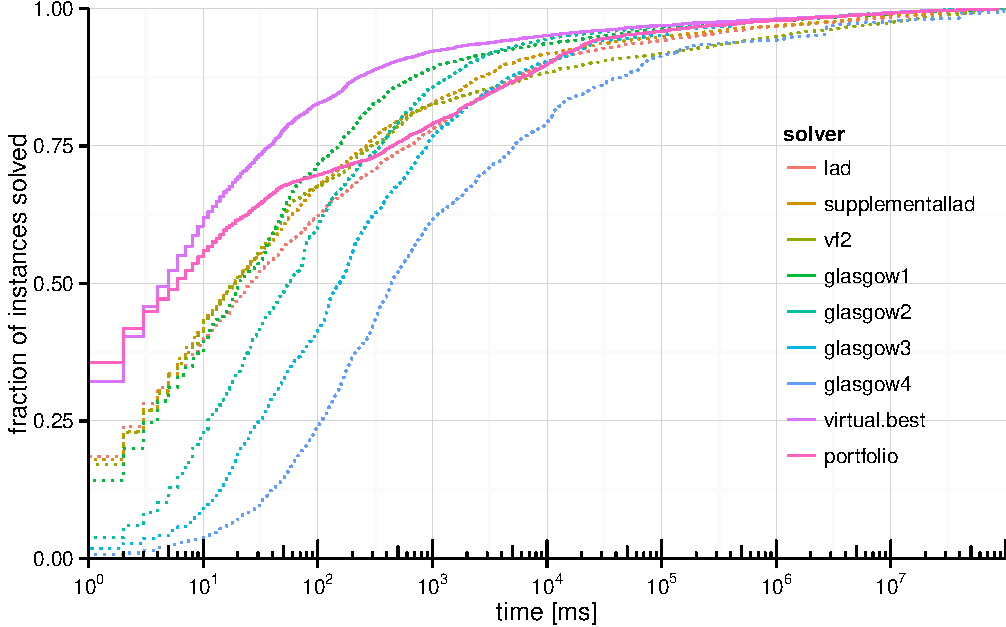
\includegraphics[width=\textwidth]{figures/portfolio-ecdf-full}
\caption{Empirical cumulative distribution function of solvers, virtual best
solvers, and the portfolio system on the full set of 5725 instances. The
actual solvers are shown as dashed lines.}
\label{fig:portfolio-ecdf-full}
\end{figure}

We train the algorithm selection model specifically for the timeout of $10^8$
milliseconds. In particular, we are interested in minimising the performance
difference to the virtual best. Problem instances that take longer to solver
contribute more to this difference than easy instances and therefore carry more
weight for the algorithm selection model. That is, choosing the wrong solver for
a hard instances is much worse than choosing the wrong solver for an easy
instance.

Even though Figures~\ref{fig:portfolio-ecdf} and~\ref{fig:portfolio-ecdf-full}
show that on easy instances, the portfolio does not perform well, it does over
the entire set of instances (cf.\ Tables~\ref{tab:res} and~\ref{tab:resfull}).

\subsection{Portfolios for Different Timeouts}

The question arises of whether the success of our approach is limited to the
particular timeout we have chosen. Table~\ref{tab:resTimeouts} shows the
performance of our portfolio for timeouts ranging from $10^2$ to $10^8$. We
do not include \IncompleteLAD and \VFtwo presolving here, as these components do not
change for different timeouts.

\begin{table}[ht]
\centering
\begin{tabular}{llrrr}
  \toprule
timeout & solver & mean MCP & solved instances & mean performance\\
  \midrule
$10^2$ & virtual best & 0 & 1253 & 59\\
 & \LLAMA & 3 & 685 & 78\\
 & \Glasgow1 & 11 & 903 & 71\\
  \midrule
$10^3$ & virtual best & 0 & 1781 & 322\\
 & \LLAMA & 22 & 1284 & 569\\
 & \Glasgow1 & 126 & 1539 & 449\\
  \midrule
$10^4$ & virtual best & 0 & 1943 & 2018\\
 & \LLAMA & 186 & 1771 & 3342\\
 & \Glasgow2 & 683 & 1855 & 2701\\
  \midrule
$10^5$ & virtual best & 0 & 2045 & 14348\\
 & \LLAMA & 1346 & 2022 & 17231\\
 & \Glasgow2 & 3019 & 1988 & 17368\\
  \midrule
$10^6$ & virtual best & 0 & 2111 & 108060\\
 & \LLAMA & 10826 & 2087 & 120459\\
 & Glasgow2 & 22729 & 2063 & 130789\\
  \midrule
$10^7$ & virtual best & 0 & 2178 & 815577\\
 & \LLAMA & 91012 & 2156 & 908200\\
 & Glasgow2 & 198944 & 2129 & 1014522\\
  \midrule
$10^8$ & virtual best & 0 & 2219 & 5822809\\
 & \LLAMA & 740765 & 2204 & 6565232\\
 & Glasgow2 & 1969418 & 2172 & 7792227\\
\bottomrule
\end{tabular}
\vspace{1ex}
\caption{Algorithm selection performance for different timeouts.}\label{tab:resTimeouts}
\end{table}

The results show that while for the misclassification penalty, \LLAMA is always
better than the single best algorithm, for timeouts $10^2$ to $10^4$ it is worse
in terms of the number of solved instances and mean performance. The
misclassification penalty does not take the cost of computing features into
account, while the mean performance does---for these small timeouts, the cost
of computing the features dominates any improvement through algorithm selection.
Another explanation for this is that empirical runtime measurements are
inherently noisy, which affects the accuracy of the measurements and hence the
performance of the algorithm selection models particularly in this range.

\begin{table}[t]
\begin{center}
\begin{tabular}{|c||r||r|r|r||r|r|r|r||r|r|}
\hline
$t$ & \VFtwo & \multicolumn{3}{c||}{LAD} & \multicolumn{4}{c||}{\Glasgow}& VBS & $\delta$\\
&&incomplete&classic&path&1&2&3&4&&\\\hline
$10^0$ & 300 &  \cellcolor{blue!25}1126 & 661 & 599 & 386 & 95 & 39 & 12 & 1132 & 6\\\hline
$10^1$ & 1699 & 1858 & 2101 &  \cellcolor{blue!25}2287 & 2061 & 1215 & 455 & 208 & 3388 & 101\\\hline
$10^2$ & 2834 & 1912 & 3376 & 3708 &  \cellcolor{blue!25}3943 & 3344 & 2295 & 1329 & 4636 & 693\\\hline
$10^3$ & 3458 & 1918 & 4233 & 4531 &  \cellcolor{blue!25}4908 & 4763 & 4262 & 3426 & 5170 & 262\\\hline
$10^4$ & 3701 & 1919 & 4888 & 5025 & 5156 &  \cellcolor{blue!25}5253 & 5022 & 4408 & 5332 & 79\\\hline
$10^5$ & 3850 & 1919 & 5108 & 5193 & 5301 &  \cellcolor{blue!25}5377 & 5292 & 5082 & 5434 & 57\\\hline
$10^6$ & 3977 & 1919 & 5244 & 5307 & 5386 &  \cellcolor{blue!25}5452 & 5451 & 5235 & 5500 & 48\\\hline
$10^7$ & 4082 & 1919 & 5336 & 5414 & 5458 & 5517 &  \cellcolor{blue!25}5518 & 5425 & 5567 & 49\\\hline
$10^8$ & 4191 & 1919 & 5423 & 5479 & 5508 &  \cellcolor{blue!25}5561 & 5560 & 5554 & 5608 & 47\\\hline
\end{tabular}
\end{center}
\caption{Number of solved instances at different CPU time limits: Each line displays a time limit
$t$ (in milliseconds) followed by the number of instances solved within this time limit by \VFtwo,
\IncompleteLAD, classical \LAD, and \PathLAD, \Glasgow with the lengths of paths limited to 1, 2, 3 and
4, and the VBS. The best single algorithm is highlighted in blue, and the difference between VBS and
single best if displayed in the last column ($\delta$).\label{expTimeTable}}
\end{table}

Table~\ref{expTimeTable} displays the number of instances solved at different CPU time limits,
ranging from 1 to $10^8$ milliseconds. It shows us that the best single solver depends on the time
limit considered. Simple approaches like \IncompleteLAD and \VFtwo are able to solve easy instances
very quickly, in a few milliseconds. However, they are not able to solve harder instances:
\IncompleteLAD is an incomplete approach which can only detect rather trivial inconsistencies; \VFtwo
performs a basic backtracking search and is very fast on easy instances, because it does not compute
expensive invariants. Classical \LAD, \PathLAD, and the \Glasgow algorithms solve more instances than \VFtwo
and \IncompleteLAD when considering longer time limits: \SI{10}{\ms} for \LAD and \PathLAD and
\GlasgowOne, and \SI{100}{\ms} (resp. \SI{1000}{\ms} and \SI{10000}{\ms}) for \GlasgowTwo (resp.\ 3 and
4). The Virtual Best Solver (VBS), which considers the best algorithm for each instance separately,
obtains much better results, showing us that the algorithms have complementary performance. The
difference between VBS and single best (column $\delta$ of Table \ref{expTimeTable}) is more
particularly important for rather small CPU time limits. In particular, VBS solves 693 more
instances than the single best (\GlasgowOne) when the limit is \SI{100}{\ms}. In many applications,
it is important to have the fastest possible algorithm. For example, in pattern recognition
applications, we often have to solve subgraph isomorphism problems for a very large number of graphs
(in order to find a pattern image in a large database of target images, for example), so that having
an algorithm that is able to solve an instance in \SI{100}{\ms} instead of \SI{1000}{\ms} makes a
big difference. Therefore, it is important to select the best algorithm for each instance.

Table~\ref{selectionvsvbs} shows the performance of our algorithm selection approach, compared to
the VBS (which is the upper bound of what an algorithm selection approach can achieve), and the
single best solver, at different CPU time limits (the single best corresponds to results highlighted
in blue in Table 1).  Comment Table 3: Mean runtime but also number of solved instances at different
CPU time limits.  Logically, \LLAMA may solve less instances than single best for small time limits
because it spends time to compute features and choose a solver, but it should be better for larger
time limits...

\begin{table}
\begin{tabular}{|l|r|rrrrrrrrr|}
&mean & \multicolumn{9}{c|}{Number of solved instances}\\
&runtime & $10^0$ &  $10^1$ &  $10^2$ &  $10^3$ &  $10^4$ &  $10^5$ &  $10^6$ &  $10^7$ &  $10^8$\\\hline
VBS & 2375.9 & 1132 & 3388 & 4636 & 5170 & 5332 & 5434 & 5500 & 5567 & 5608\\\hline
Single best & 3177.6 & 1126 & 2287 & 3943 & 4908 & 5253 & 5377 & 5452 & 5518 & 5561\\\hline
\LLAMA & 2706.3\\\hline
\end{tabular}
\caption{}\label{selectionvsvbs}
\end{table}

Add Figure 1 which compares single best at \SI{e8}{\ms}(\GlasgowTwo) with \LLAMA ?

\section{Conclusion and Future Work}

The problem of identifying subgraph isomorphisms is a hard computation problem
that has many applications in diverse areas. In this paper, we presented a
portfolio of six algorithms from the literature and a novel variant of the \LAD
algorithm. We introduced a set of novel features to characterise subgraph
isomorphism problems and leveraged them to select the most appropriate algorithm
from the portfolio for each instance.

We demonstrated that our portfolio achieves substantial performance improvements
over the single algorithm that has the best performance on our benchmark set. We
showed that combining a portfolio approach with a novel incomplete variant of
\LAD that is able to detect inconsistencies and a presolver boosts performance
even further.

Mention parallel, directed, labelled in here briefly.

\bibliographystyle{splncs}
\bibliography{paper}

\end{document}

